\documentclass{article}
\usepackage[utf8]{inputenc}
\usepackage[english]{babel}

\usepackage[
backend=biber,
style=alphabetic,
citestyle=authoryear
]{biblatex}
\addbibresource{bibliography.bib}
\usepackage{graphicx}
\usepackage{caption}
\usepackage{subcaption}
\usepackage{hyperref}
\title{Interim report: Mellon}
\author{Neele Falk }
\date{November 2020}
\setlength{\parindent}{0pt}
\begin{document}

\maketitle

\section{Work Package 2. LAPPS/CLARIN Integration}
\subsection{Full interoperability within WebLicht -- conersion between dataformats}
To enable a seamless workflow between all data exchange formats in the LAPPS-CLARIN framework, a conversion between the different data exchange formats has to be implemented. Within the first project a conversion between the LAPPS format LIV \parencite{liv} and the Weblicht format Tcf \parencite{Tcf} has already been implemented successfully. \parencite{firstphase} A missing part to achieve the goal of full interoperability is the conversion between Tcf and Conll-U. Until now, both formats have been integrated into WebLicht through a variety of services, but the services can not be combined into a mixed pipeline according to the mix and match principle. To complete the work started in the first project, converters from Conll-U to Tcf and vice versa were added as 'services' to the LAPPS-CLARIN framework.

\textbf{Conll-U2Tcf}

Although the Conll-U services are subdivided into several smaller services (1) UDPipe tokenizer: produces tokens, (2) UDPipe tagger: produces part-of-speech tags, lemmas, morphology, (3) UDPipe parser: produces dependency relations, we only allow a conversion to Tcf after all Conll-U services have been run. It would have been possible to add three converter services that match the output of each Conll-U service. But because a converter always overwrites the output of the previous service, the user would have been able to overwrite a richer annotated document with a Tcf containing less annotations by using the wrong converter. The Conll-U converter can be run after the three Conll-U services have been applied to an input document. Any WebLicht service that is based on Tcf can afterwards be applied to the input document to add, for example, named entities. Or, to complete the cycle, the Tcf can then be converted to LIV to apply a LAPPS service.

Using the Conll-U format, the converter can internally detect which annotations are present. If an annotation is not present in Conll-U, this column is marked with an underscore. A challenge with this converter was the fact that not all existing annotations could be transferred from Conll-U to Tcf. For example, Conll-U contains two annotation layers for part-of-speech tagging: a language-specific and a universal one, whose schema is defined the same for all languages. In Tcf, only one annotation layer per annotation type is possible. We have decided to adopt the layer according to the universal annotation scheme, since it is consistent for all languages. 
 

\subsection{Integrating new services into WebLicht for named entity recognition}
The recent progress in the field of computational linguistics, especially the development of systems that are based on neural networks, has led to large improvements in most natural-language processing tasks. To achieve our goal of enriching the metadata of archive data with named entities, we have added new services for named entity recognition to WebLicht based on deep learning architectures. The services output 
\begin{itemize}
    \item \textbf{sticker 1 \footnote{\hyperlink{https://github.com/stickeritis/sticker}{https://github.com/stickeritis/sticker}}}: this service is a sequence labeler that can be used to perform any sequence labeling task in principle. The named entity recognition can be formulated as a sequence labeling task, each token being annotated with a tag of the BIO schema. In this schema a token can be annotated with an O (not part of a named entity), a B (first token of the named entity) or an I (a token within a named entity). sticker 1 can use recurrent neural networks, transformers or dilated convolutional networks.
    \item \textbf{sticker 2 \parencite{sticker2}}: the sticker service was further improved by integrating the latest state-of the art techniques, such as pretrained transformer networks \parencite{xmlroberta} and multi-task learning. It can be viewed as a 'superservice' as it outputs multiple annotations at once. Thus, the underlying architecture can benefit from being trained on several different, but related tasks (e.g. pos-tagging and dependency parsing). 
\end{itemize}

\section{Worpackage 3 and 4: Enriching metadata with named entities}

To facilitate the search and analysis of large corpora for researchers from other fields (e.g. digital humanities, political science) and to make the information from these corpora usable, we have developed a pipeline that enriches the metadata of such corpora and outputs them in a structured format. 
Within the pipeline, the existing metadata are automatically extracted and additional information about named entities are leveraged by using the previously described state-of-the art services that have been integrated into the LAPPS-CLARIN framework. The named entities are automatically linked to a unique identifier using authority records for persons and georeferences for locations. The output of the pipeline are CMDI records, that store this metadata in a structured way which is consistent across the different sub corpora and well defined. 

\subsection{GermaParl}

The German part of the German and Czech Parliamentary proceedings (GCPP), GermaParl \parencite{germaparl}, has been prepared as part of the PolMine Project (https://polmine.github.io/) based on the protocols of plenary debates published by the German Bundestag. 
The corpus, being indexed and consolidated, is available as an XML-based format (TEI). It contains some general metadata, such as the legislative period, the date and the number of plenary protocol. Within the TEI there is also more fine-grained metadata: each speech event is annotated with a speaker, each speaker is annotated with a role, position and party. Figure \ref{fig:TEI} shows an example TEI of the corpus with the highlighted metadata. The GermaParl corpus contains more than 100 million tokens.
\begin{figure}
\centering
\begin{subfigure}{0.5\textwidth}
  \centering
  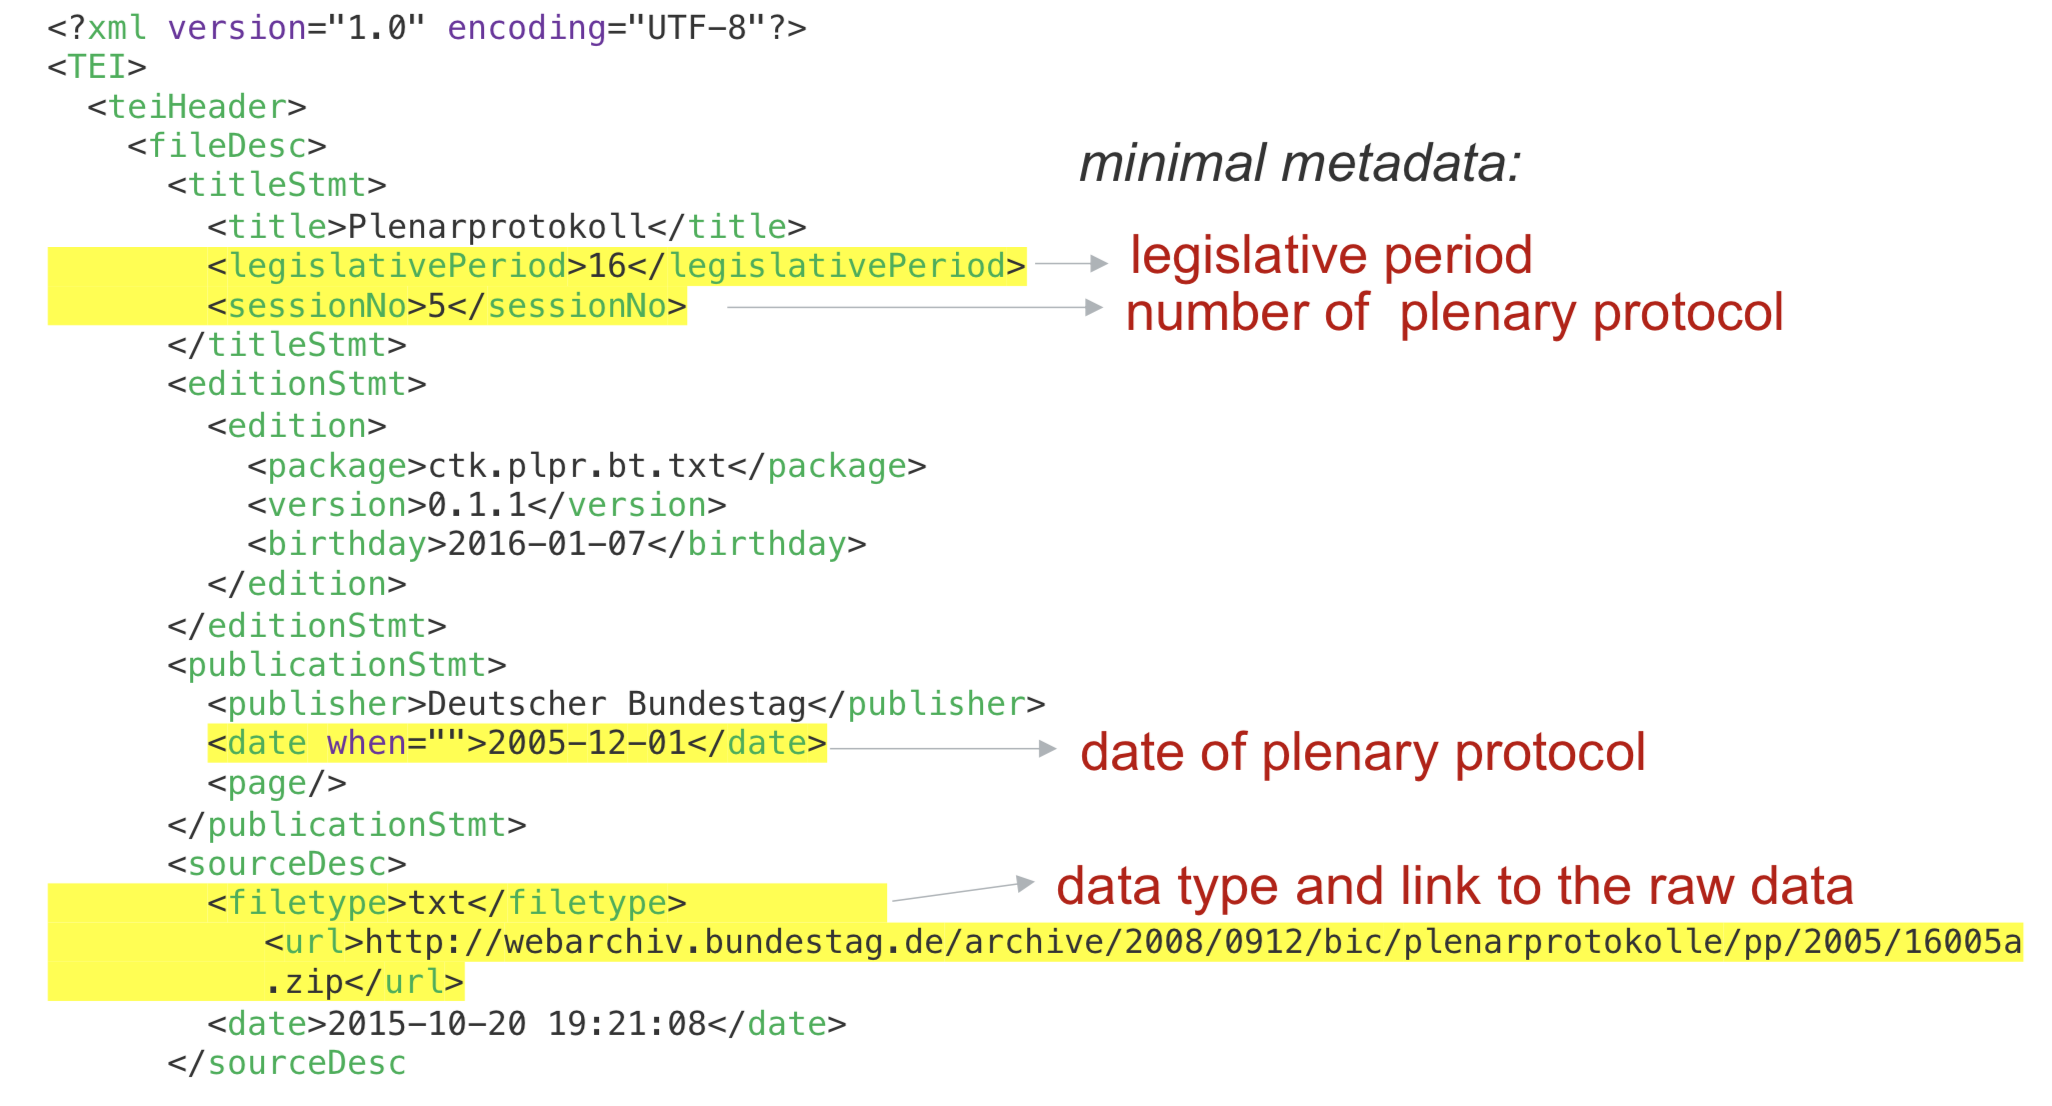
\includegraphics[width=\textwidth]{tei1.png}
  \caption{Header of the TEI with general metadata}
  \label{fig:sub1}
\end{subfigure}%
\begin{subfigure}{0.5\textwidth}
  \centering
  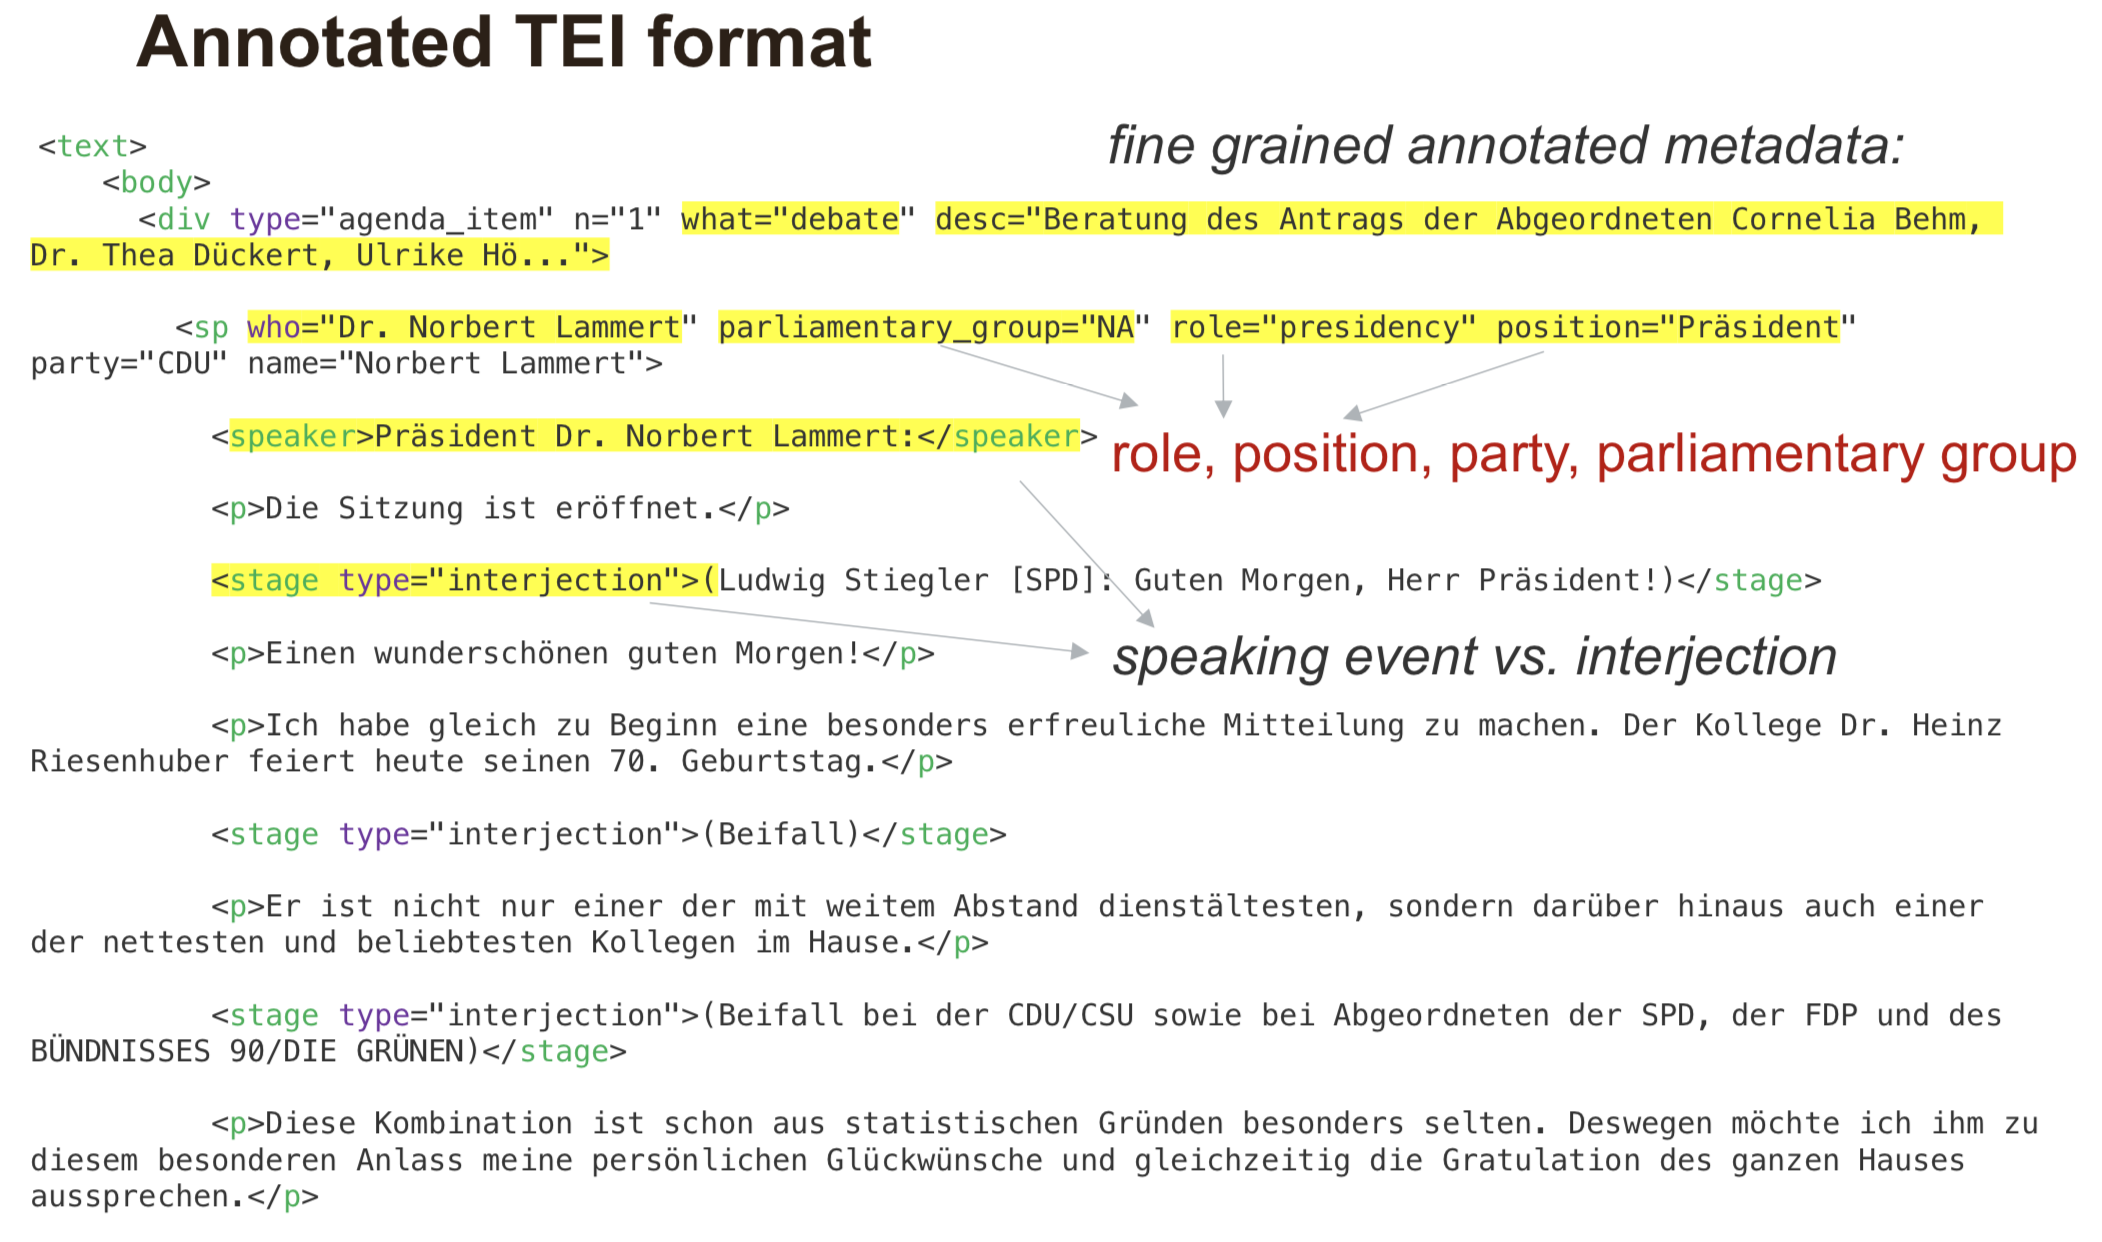
\includegraphics[width=\textwidth]{tei2.png}
  \caption{Example speech event with specific metadata form TEI}
  \label{fig:sub2}
\end{subfigure}
\caption{Example of XML-based TEI form GermaParl}
\label{fig:TEI}
\end{figure}

\subsubsection{Authority files}
Authority files are databases that contain a distinct numeric identifier for persons, organizations or geographical locations. The authority files contain links to other authority file identifiers and other databases (e.g. Wikipedia). They also contain metadata, e.g. nationality and occupation of a person. We are working with the virtual international authority file (VIAF), that contains organizations and people. This authority control combines several national authority files (e.g. it contains the data from the German national library (DNB)). For geographical entities we use the database GeoNames. 
To extract the persistent identifiers of the authority files, we use the Virtual International Authority File (VIAF) API which allows to search the authority database by keyword, preferred name or control number. Having an automatically extracted named entity, we use a SRU search query to search for matching authority source records. We also try the autosuggest functionality which provides a fast lookup for eventually incomplete or incorrectly spelled names. An example VIAF entry for the person 'Angela Merkel' is displayed in figure \ref{fig:agenlamerkel}, showing the unique persistent idenfifier (VIAF ID), the nationality and occupation and links to other authority records and databases (e.g. Wikipedia).
\begin{figure}
    \centering
    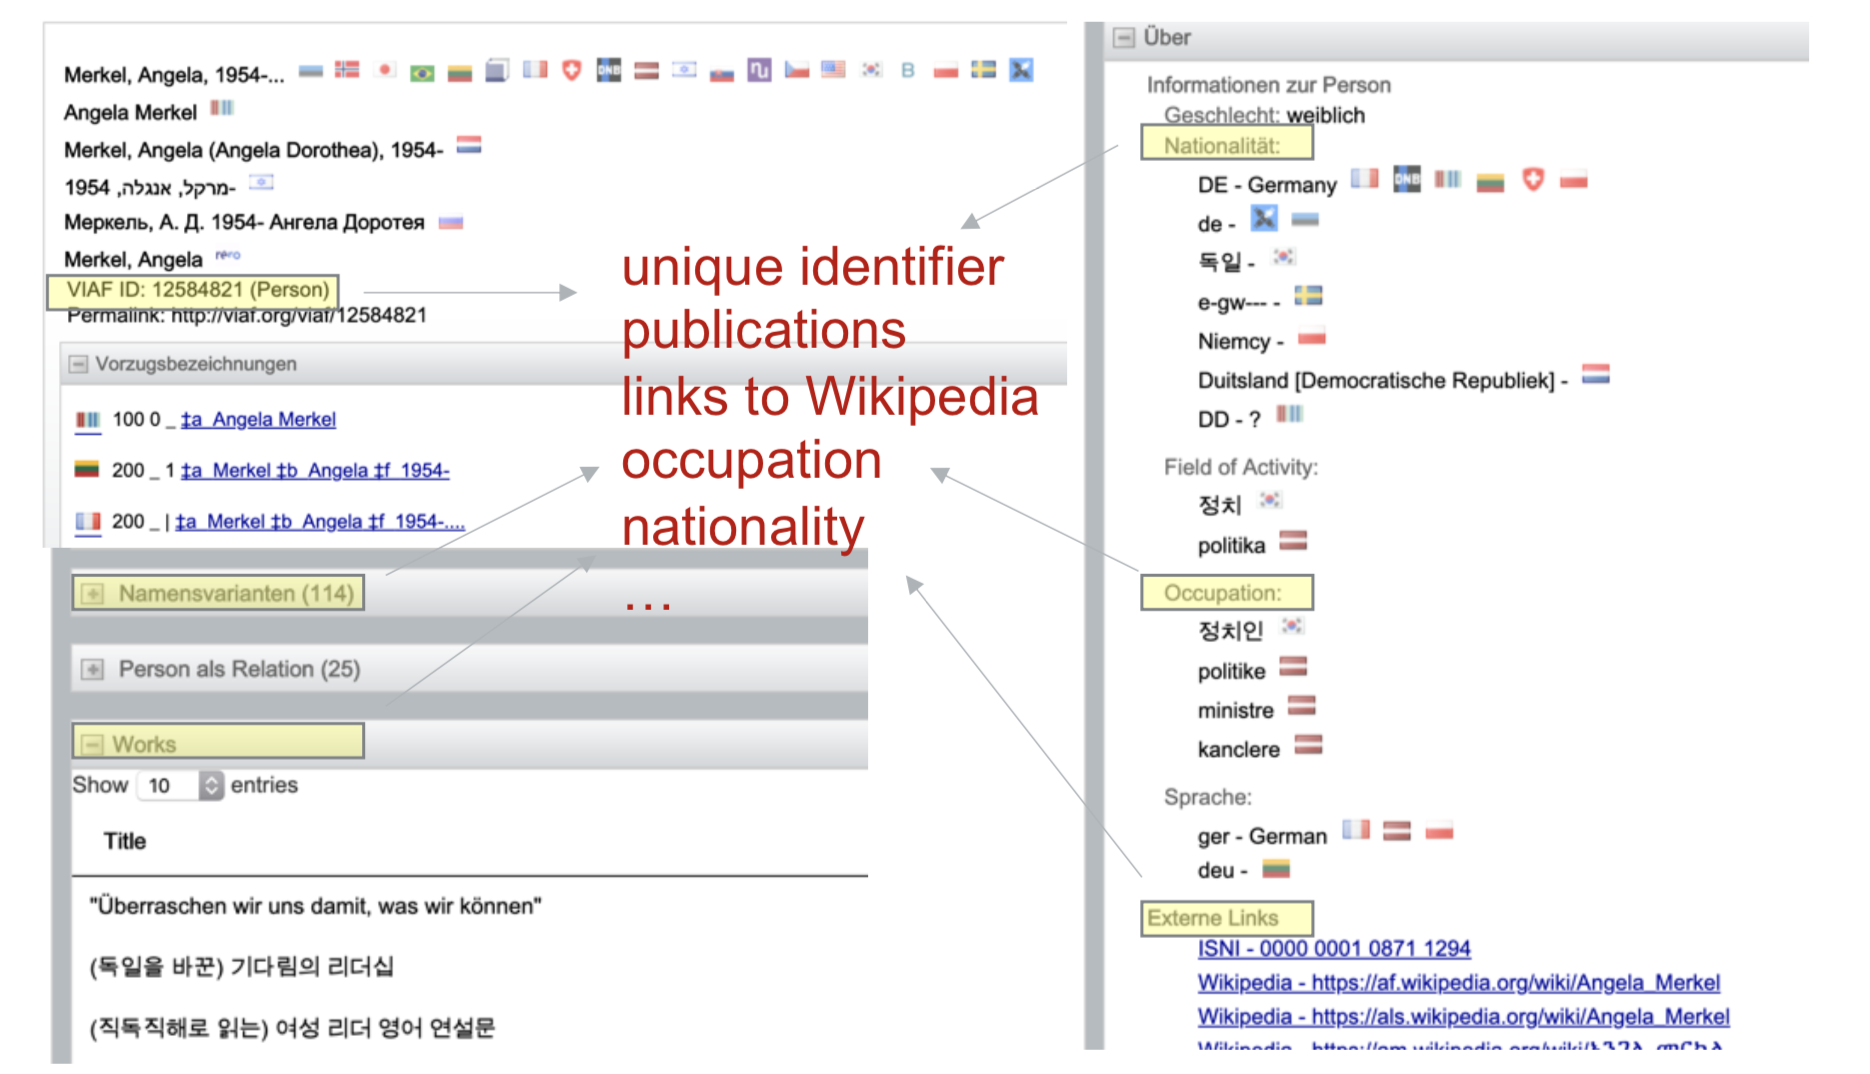
\includegraphics[width=\textwidth]{angela.png}
    \caption{Example VIAF entry 'Angela Merkel'}
    \label{fig:agenlamerkel}
\end{figure}

\subsubsection{Pipeline}
The following proveds an overview of the processing pipeline that has been executed to enrich the metadata of the GermaParl archive.
\begin{enumerate}
    \item extract existing metadata from XML
    \item extract raw text for each speech event from XML
    \item tokenize the raw text with the \href{http://hdl.handle.net/11022/0000-0007-E7D0-9}{German Somajo Tokenizer service}\footnote{\href{http://hdl.handle.net/11022/0000-0007-E7D0-9}{http://hdl.handle.net/11022/0000-0007-E7D0-9}}
    \item extract named entities with the \href{http://hdl.handle.net/11022/0000-0007-DA29-6}{sticker named entity recognition service} service\footnote{\href{http://hdl.handle.net/11022/0000-0007-DA29-6}{http://hdl.handle.net/11022/0000-0007-DA29-6}}
    \item extract candidate VIAF IDs and IDs from GeoNames for persons, organizations, locations and geographical entities
    \item create CMDI records with the extracted metadata
\end{enumerate}
\begin{figure}
    \centering
    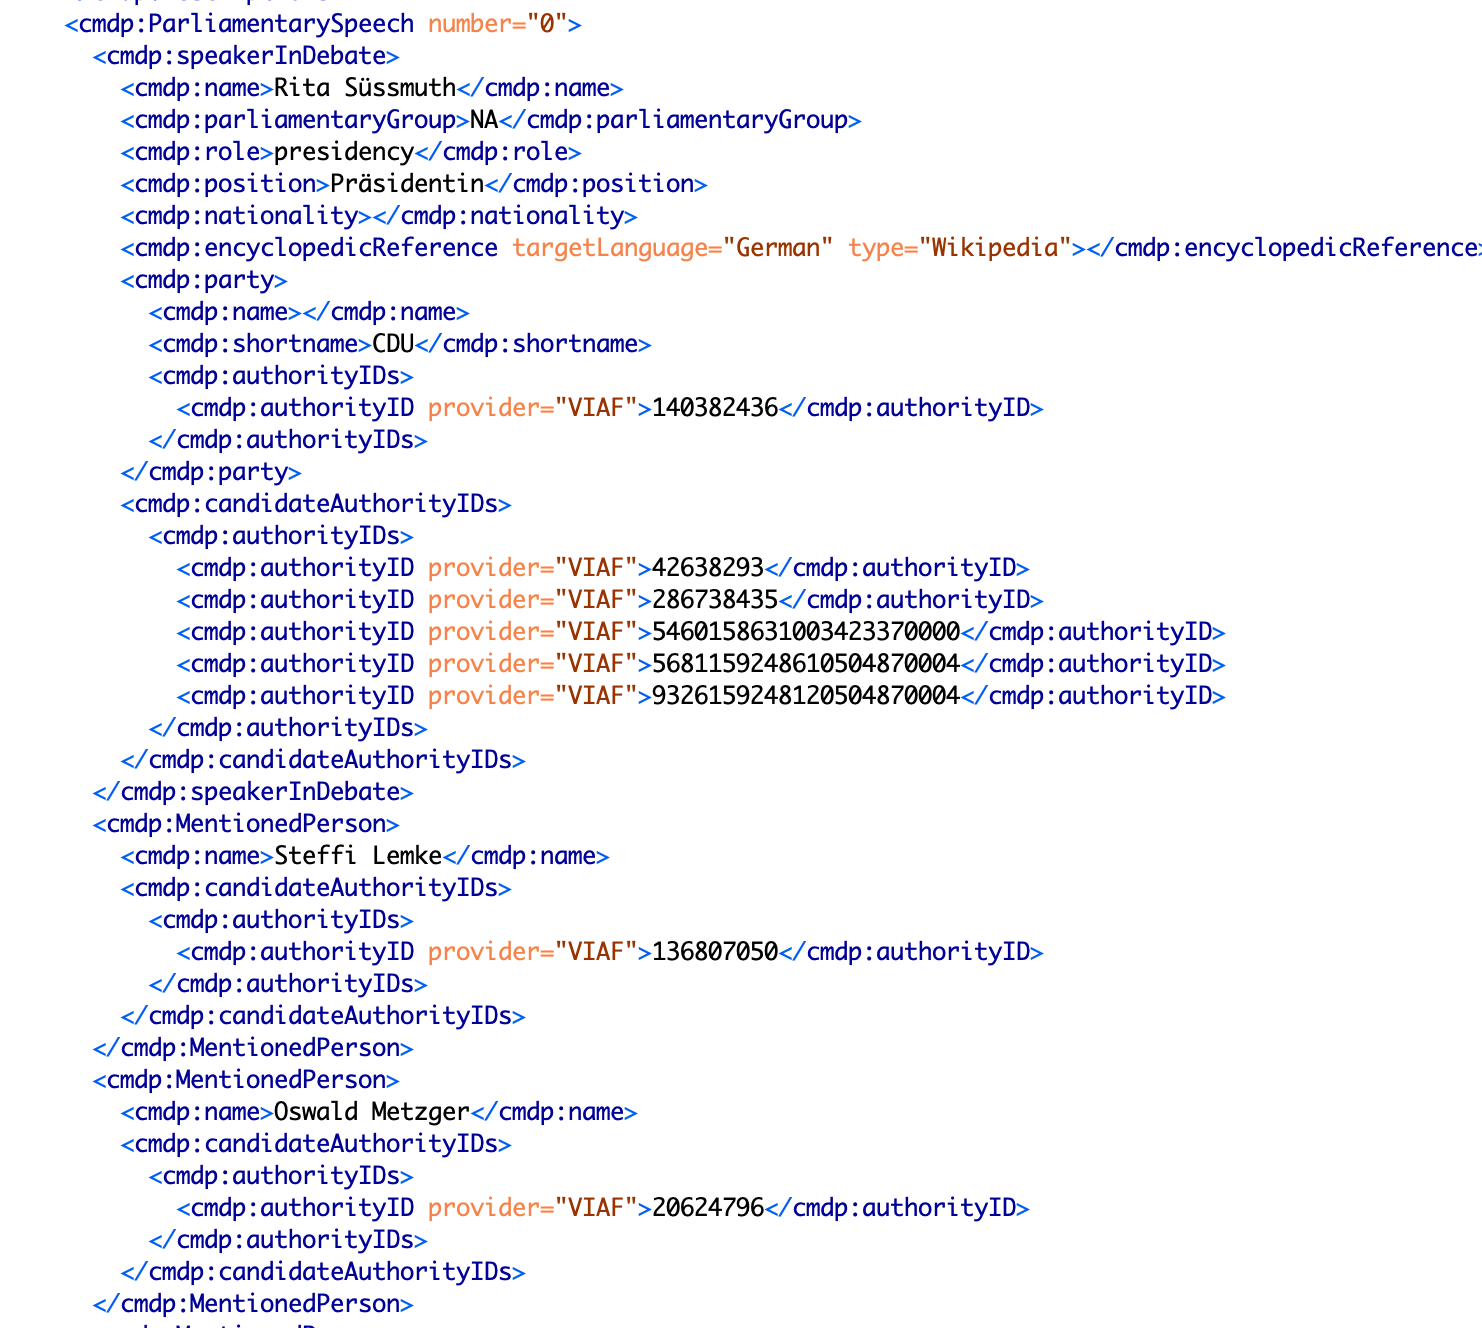
\includegraphics[width=\textwidth]{cmdi1.png}
    \caption{Example from output CMDI}
    \label{fig:cmdi}
\end{figure}
In the example CMDI record (see figure \ref{fig:cmdi}) the structure of the metadata is visualized. Each debate is divided into several parliamentary speech items, each speech event is associated with a specific numner and a specific speaker (speakerInDebate). In this case the speaker, Rita Süssmuth has a role (presidency) and a party (CDU). The party has a unique authority ID, extracted from the VIAF authority database. Table \ref{tag:entity_freq} shows the most frequent mentioned persons, locations and organizations in the corpus.

Besides the metadata, we provide an interactive script to search the metadata for information of interest. For example, one can search for a specific entity to retrieve all documents the entity occurs in, the number of times the entity occurs in each document and the total frequency. On top of that the script can output VIAF IDs and other metadata, such as role or corresponding parties for specific entities. In a more detailed view (compare figure \ref{fig:cmdiextractor}, the query was 'Angela Merkel') each document of interest is listed with the corresponding mentioned persons, locations and organizations. This functionality can for example be used to find all the documents or speech events a person (e.g. Angela Merkel) has talked about a certain entity (e.g. where did she talk about Syria or the NATO). One can also get a list of all persons, organizations and locations, existing in the corpus. As a future step the script can be converted into a Webservice to facilitate the use for researches from humanities. 
\begin{figure}
    \centering
    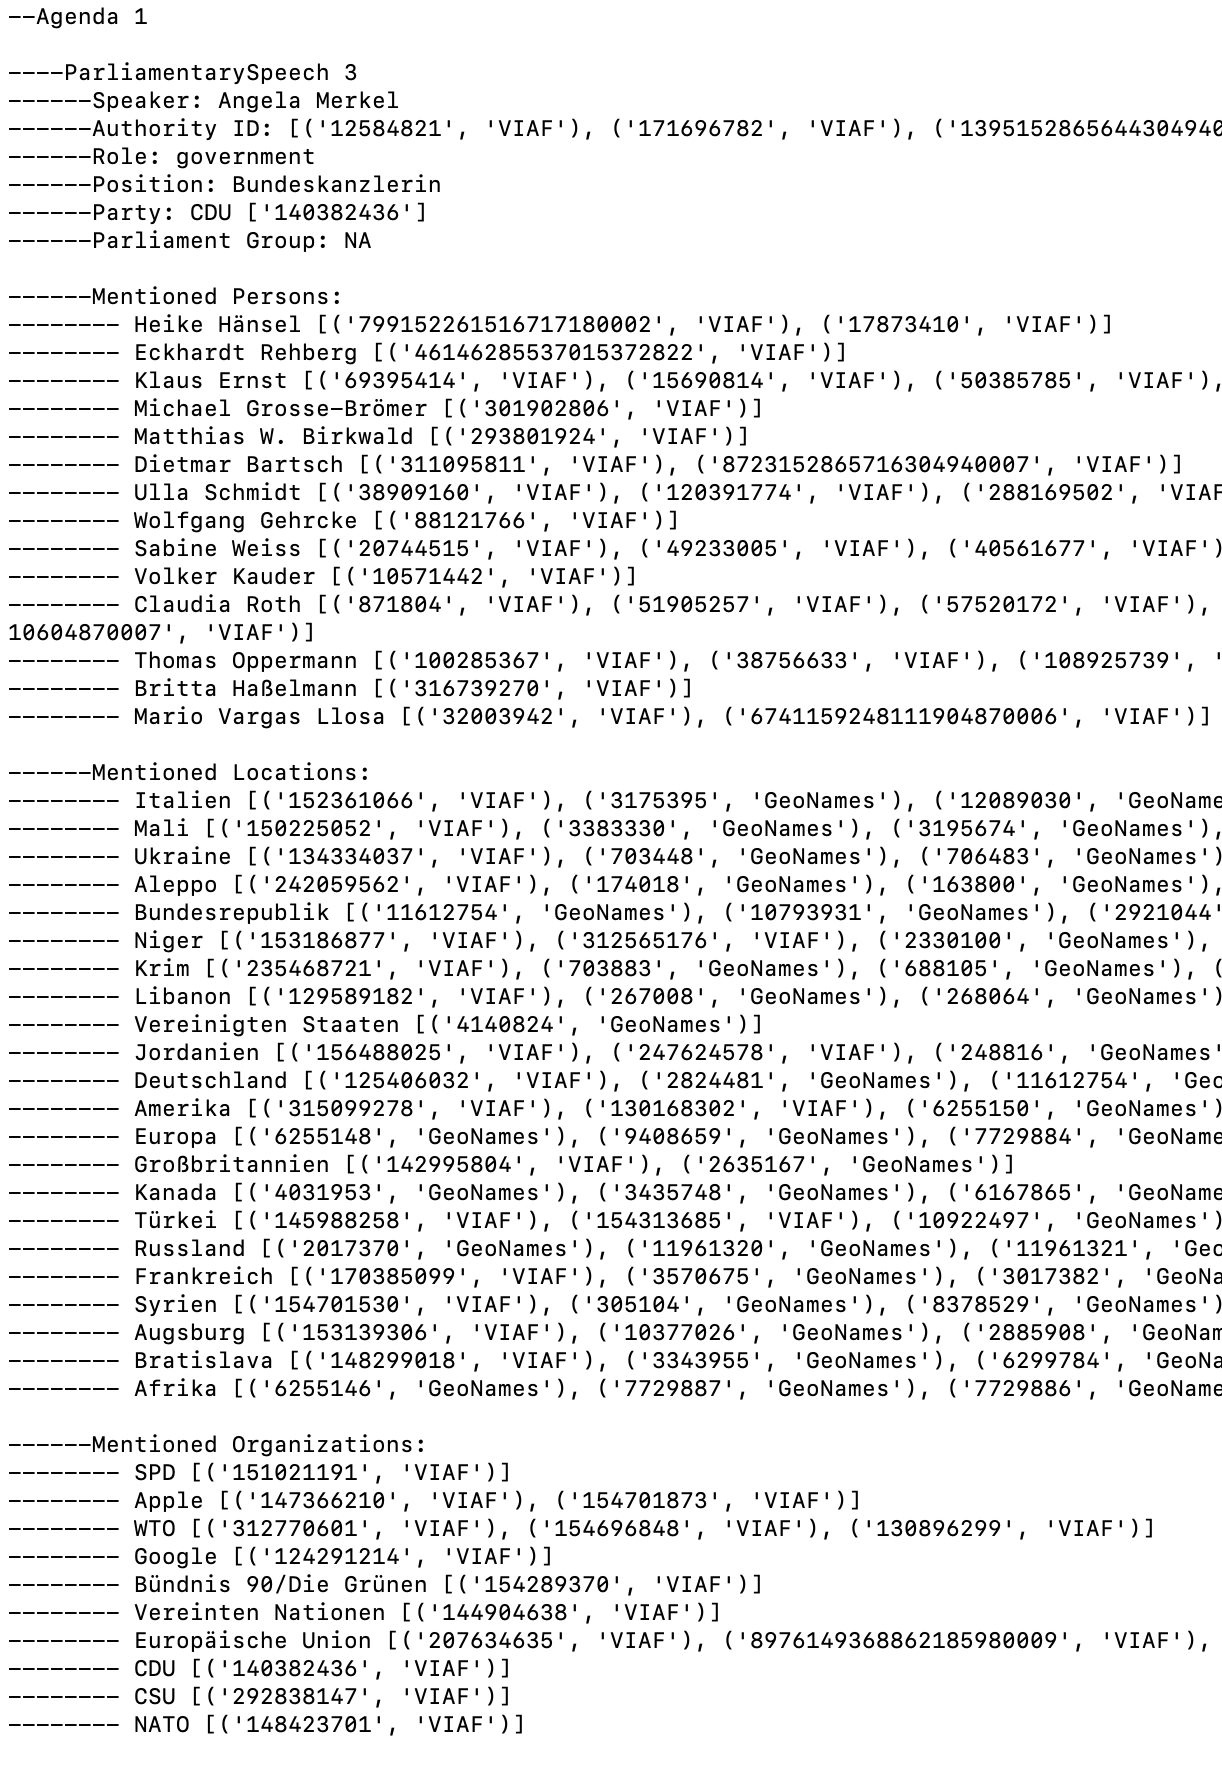
\includegraphics[width=\textwidth]{cmdiextractor.png}
    \caption{Example output of the cmdi extractor, detailed view, for the query 'Angela Merkel'}
    \label{fig:cmdiextractor}
\end{figure}
\begin{table}[h!]
\resizebox{\columnwidth}{!}{
\begin{tabular}{|lr|lr|lr|}
\hline
\multicolumn{2}{|l|}{\textbf{person}}  & \multicolumn{2}{|l|}{\textbf{location}} & \multicolumn{2}{|l|}{\textbf{organization}}  \\\hline
\textbf{name}   & \textbf{frequency} & \textbf{name}   & \textbf{frequency}  & \textbf{name}         & \textbf{frequency} \\\hline
Volker Beck     & 4,032              & Deutschland     & 49,288              & CDU                   & 104,913            \\
Jörg Tauss      & 3,595              & Europa          & 14,908              & CSU                   & 99,795             \\
Volker Kauder   & 3,050              & Berlin          & 10,004              & SPD                   & 95,671             \\
Wilhelm Schmidt & 2,917              & Bundesrepublik  & 8,244               & Die Grünen & 55,129             \\
Dirk Niebel     & 2,681              & USA             & 6,332               & FDP                   & 50,112          \\  \hline
\end{tabular}}
\caption{Top 5 most frequent mentioned entities in GermaParl}
\label{tag:entity_freq}
\end{table}
\subsubsection{Evaluation}
In order to verify that reasonableness of our approach, we developed a small evaluation setup. In this setup we extracted a random dataset for each named entity type which we manually analyzed with respect to its extracted VIAF identifiers. 

\begin{table}[h!]
\resizebox{\columnwidth}{!}{
\begin{tabular}{|l|cc|cc|cc|cc|}
\hline
\textbf{entity type}             & \multicolumn{2}{|c|}{\textbf{PERS}} & \multicolumn{2}{|c|}{\textbf{LOC}} & \multicolumn{2}{|c|}{\textbf{GPE}} & \multicolumn{2}{|c|}{\textbf{ORG}} \\\hline
                                 & automatic        & verified       & automatic       & verified       & automatic       & verified       & automatic       & verified       \\\hline
\textbf{unique VIAF ID}          & 57               & 56             & 39              & 34             & 40              & 40             & 22              & 22             \\
\textbf{several VIAF IDs}        & 33               & 32             & 26              & 25             & 22              & 22             & 30              & 26             \\
\textbf{no VIAF IDs}             & 10               & 7              & 35              & 16             & 38              & 12             & 48              & --             \\\hline
\textbf{total}                   & 100              & 95             & 100             & 75             & 100             & 74             & 100             & 48             \\\hline
\textbf{at least one correct ID} & \multicolumn{2}{|c|}{88}            & \multicolumn{2}{|c|}{59}           & \multicolumn{2}{|c|}{62}           & \multicolumn{2}{|c|}{48}          
\\\hline
\end{tabular}
}
\caption{Results for automatic VIAF ID extraction for the 4 sample datasets}
\label{tab:overallresults}
\end{table}
Table \ref{tab:overallresults} display the overall results for each sample dataset. The best results were obtained for persons: for a total of 88 persons, the correct VIAF ID is among the candidate VIAF IDs, for 56 persons, a single correct VIAF ID was extracted.
Analyzing potential sources of error for this category revealed that the information in the authority file sometimes is outdated (e.g. when a person got married) or that persons were not recognized correctly by the named entity recognizer.

The named entity tags for locations are divided into two categories: GPE (Countries, cities, states) and LOC (Non-GPE locations, mountain ranges, bodies of water). For Locations the approach also works well in terms of precision, i.e. the correct VIAF ID is almost always under the candidate IDs). However the recall is lower than for persons: For a third of the locations in the two datasets, no VIAF ID was extracted.For this type of named entity we also explored a different API (Geocoder) to retrieve an ID from a different database: the GeoNames geographical database. This database is not connected to the VIAF and focuses on geographical entities only.  Table \ref{tab:geonames} shows the results for that database for each the tags LOC and GPE. We can see an improvement in the precision (66 and 72 correct IDs were extracted) but this comes with an increase in ambiguity (~ for 60 locations several IDs were extracted). The most frequent source of error for this entity type stemmed from an incorrect named entity recognition. The fact that the locations are more often declined (e.g. "Rheines" instead of "Rhein") also results in an incorrect ID extraction.


\begin{table}[h!]
\begin{tabular}{|l|cc|cc|}
\hline
\textbf{entity type}             & \multicolumn{2}{|c|}{\textbf{LOC}} & \multicolumn{2}{|c|}{\textbf{GPE}} \\\hline
                                 & automatic       & verified       & automatic       & verified       \\\hline
\textbf{unique GeoNames ID}      & 9               & 7              & 5               & 4              \\
\textbf{several GeoNames IDs}    & 67              & 59             & 72              & 66             \\
\textbf{no GeoNames IDs}         & 24              & 10             & 23              & 2              \\
\textbf{total}                   & 100             & 76             & 100             & 70             \\\hline
\textbf{at least one correct ID} & \multicolumn{2}{|c|}{66}           & \multicolumn{2}{|c|}{72}       
\\\hline
\end{tabular}
\caption{Results for automatic GeoNames extraction for the LOC and the GPE dataset}
\label{tab:geonames}
\end{table}
The most difficult named entity type are organizations. For almost half of the dataset no VIAF ID was extracted, at the same time it was hard to manually verify whether the extraction failed because of any drawback within the pipeline or because there is no existing VIAF ID for a specific organization. This was because organizations are often abbreviated. These acronyms complicate the VIAF extraction because they are too general (e.g. "Ausschuss für Arbeit und Soziales") or not meaningful enough to be mapped to specific candidate authority records. It is also difficult to manually verify such acronyms unless the annotator has a very deep knowledge of organizations and their abbreviations within the political context. For this category the named entity recognizer also had the highest error rate: 17 extracted organizations were misclassified as organizations (e.g. "Felix" or "Bahnprotest"). 
\clearpage
\nocite{*}
\printbibliography
\end{document}
